%!TEX root = ../thesis.tex
%*******************************************************************************
%****************************** Sixth Chapter **********************************
%*******************************************************************************

\chapter{Biorealistic Computing}

\section[Spiking Deep Networks]{Spiking Deep Networks}

Traditional neuromorphic circuits consist of two main components: neurons and synapses \cite{mead1989analog}. Neurons are active devices that act as decision-making units. When the input threshold is surpassed, an acceptable condition is met, and a voltage spike is generated. Synapses are usually passive elements that connect neurons with each other. This is also where primary calculations of the inputs are performed, as well as a potential storage mechanism.\\

\noindent The neurons and synapses are linked to create a neural network, which is used in all modern machine learning methodologies. Rather than responding to continuous signals, these networks communicate information through spikes. Spike trains convey data in both the form and timing of the spike, making them ideal for implementing synaptic learning principles. It is worth noting that this method adheres to the typical framework within the field, however, it presents a highly simplified conception of the biological system.\\

\noindent Modern artificial neural networks and neuro-computing architectures usually neglect the principles of neuroscience \cite{pfeiffer2018deep}. As a consequence, essential elements of the organic cerebral processing systems are either disregarded or overlooked. The aim of biorealistic approaches is to mimic the functions of computational cells using electronic devices. The creation of these circuits in CMOS was traditionally known as neuromorphic engineering, with backpropagating networks being a more direct influence from nature.

\subsection[Neural Computing Nomenclatures]{Neural Computing Nomenclatures}

Deep artificial neural networks (DNNs), particularly convolutional neural networks, represent a significant triumph in the field of modern computer vision. They have demonstrated remarkable efficacy in recognizing a diverse array of objects within expansive, intricate images \cite{krizhevsky2012imagenet}. However, these networks have been engineered for and operate exclusively on rate-based neurons. The question of how they can be executed on spiking neurons represents an emerging frontier of investigation.\\

\noindent The question arises as to why such networks should be run in spiking neurons. There are two principal motivations behind the creation of deep spiking networks. The first is to enable the operation of some of the large CNN models that have recently demonstrated success in numerous object recognition and other tasks on spiking neuromorphic hardware. This will facilitate the development of energy-efficient systems capable of performing object recognition in real time on robotic platforms, where current technology is too energy-intensive to allow for deployment on mobile robots, for example. \\

\noindent The second motivation is to incorporate additional brain-like components into machine learning models. The field of neuroscience presents a multitude of distinctive challenges pertaining to the mechanisms of learning in the brain. These include the complexities associated with the nonlinear characteristics of neurons, particularly in relation to their firing thresholds, as well as the intricacies of spike-based communication and its inherent discreteness and variability. \\

\noindent Although the spiking deep networks presented in this chapter are not designed to be models of brain-like learning processes, the challenges addressed here are also faced by the brain. Some of the ideas presented in this section provide insights that motivate the development of more biologically plausible learning mechanisms.\\

\noindent Spiking deep networks facilitate the transmission of information between neurons in the form of discrete spikes. The initial distinction to be made regarding spiking networks is that they encompass an additional temporal dimension, which is not typically present in rate-based DNNs. In other words, a spiking neuron is a process that evolves over time, sometimes emitting spikes, sometimes not.\\

\noindent It is only possible to discuss this process over time; examining it in one instant provides little insight. In contrast, in rate-based networks, we typically present an input and can instantaneously determine the activities of each subsequent neuron in the network, since they do not change over time. \\

\noindent A second notable distinction is that spikes are discrete and identical in nature. The sole information conveyed by a spike is the time at which it occurred. As previously discussed, this indicates that there are two principal categories of codes that a neuron can utilise: rate codes and timing codes. \\

\noindent In the case of a timing code, the focus is on the times of individual spikes. In contrast, if a rate code is employed, the focus shifts to the number of spikes occurring within a specific time window, or potentially the relative timing of spikes in relation to one another. \\

\noindent When examining the number of spikes within a specified time interval, it becomes evident that the resulting rate is inherently discrete. If there are \textit{n} spikes within the \textit{t}-second window, the firing rate can be expressed as \textit{n/t}, where \textit{n} is an integer. For a fixed window \textit{t}, the firing rate can only assume a discrete set of values, specifically all the integer values of \textit{n}. \\

\noindent A third distinction pertains to the inherent variability of the output of spiking neurons, which differs from that of their rate-based counterparts. In the event of a constant input, a rate neuron will provide a constant output, that is to say, the firing rate corresponding to that input. \\

\noindent It should be noted that rate neurons are capable of exhibiting internal dynamics, as exemplified by the adapting version of the rate-based LIF. Consequently, when presented with a constant input, the output of these neurons will not be constant. Nevertheless, their output remains considerably less variable than that of their spiking counterparts. \\

\noindent In contrast, spiking neurons will output a spike train, which, when filtered by a synapse, results in an oscillating signal whose variability depends on the firing rate. Consequently, even when presented with a constant input, a spiking network will exhibit variability in the inputs to each neuron and the outputs of the entire network. \\

\noindent DNNs are typically formulated as rate-based models, wherein the nonlinearity activity is understood to represent the firing rate of a neuron. To illustrate, a ReLU can be conceptualised as a neuron that is silent in the event that its input is less than zero, and whose firing rate increases in a linear fashion as the current rises above zero. \\

\noindent Moreover, cost functions associated with rate-based DNNs are based on the firing rates of the output neurons. In the context of classification, the chosen class is the output unit with the highest activity. One approach is therefore to treat spiking networks similarly and train the network so that the unit corresponding to the target class will have the highest activity. \\

\noindent It should be noted that this activity does not necessarily correspond to a neuron firing rate. Indeed, it is more likely to be the filtered, weighted sum over the spiking activities of the final layer of neurons in the network. Alternatively, the network can be trained so that the first neuron to spike will be the chosen class.\\

\noindent At the level of a single neuron, this distinction is no longer applicable. The activity of a neuron firing at a regular rate can be captured by its inter-spike interval, defined as the time between one spike and the next. Assuming the neuron is in a resting state, the inter-spike interval is equivalent to the time before the first spike of a neuron, plus the refractory period. The key design decision is how information is transmitted between neurons.

\subsection[Memristive Frameworks]{Memristive Frameworks}

\noindent Modern deep learning algorithms are subjected to neuroscience-inspired restrictions by Spiking Neural Networks (SNNs) \cite{tavanaei2019deep}, which have shown notable increases in runtime efficiency \cite{wang2020supervised}. Neuromorphic hardware has demonstrated considerable reductions in latency and energy consumption \cite{wunderlich2019demonstrating}, by switching from full precision and fixed precision activations of artificial neuron models to temporally-encoded data representations collected by spiking neurons \cite{zhou2020towards}.\\

\noindent The considerable success of error backpropagation in training deep learning models has led to the development of numerous related training algorithms tailored for spiking neural networks (SNNs) \cite{werbos1990backpropagation}. These algorithms, which are guided by surrogate gradient descent, have been designed to address the non-differentiability of discrete spikes, which is a limitation of traditional gradient-based methods \cite{neftci2019surrogate}. This proliferation of SNN usage is accompanied by the development of modular deep learning programming packages \cite{hazan2018bindsnet} that have optimised autodifferentiation for CUDA acceleration \cite{pehle2021norse}. \\

\noindent In parallel with these advances in training SNNs, the past decade has seen significant developments in brain-inspired devices, circuits, and architectures that integrate neuronal dynamics to enhance the hardware integration of SNNs and their constituent parts. Memristors and resistive RAM (RRAM) constitute a significant aspect of the exploratory research conducted in the field of SNN implementation \cite{chua1971memristor}, as they serve as a natural conduit between SNN algorithms and accelerators \cite{chua1976memristive}. They have been extensively utilized as both synapses and as spiking neurons. \\

\noindent At the ionic level, memristive synapses have been integrated into systems that naturally implement the spike-timing-dependent-plasticity (STDP) update rule using higher-order device dynamics \cite{serrano2013stdp}, as evidenced by the literature \cite{lin2020adaptive}. An alternative application of ion-driven dynamics is the implementation of the memristor as a neuron, where nonlinear conductance evolution gives rise to abrupt switching that can be used to emit sudden voltage spikes \cite{lim2015reliability}.\\

\noindent This approach \cite{bao2019dual} is typically coupled with capacitive integration and has been referred to as a 'neuristor' \cite{del2020caloritronics}, and a 'Memristive Integrate-and-Fire' (MIF) neuron \cite{hao2020monolayer,kang2021build,zhou2022fully}. Similarly, the leakage of ions through the membrane of biological neurons can be implemented using resistive dissipation \cite{loeffler2021modularity}, as in neuristors, as observed in nanowire networks \cite{hochstetter2021avalanches,zhu2021mnist}, or via the dynamic movement of ions in single devices \cite{zhu2020memristor}. \\

\noindent At the architectural level, RRAM has been identified as a promising candidate for in-memory compute (IMC) architectures \cite{li2018analog} due to its capacity to parallelise matrix-vector multiplication independently of time complexity when integrated as large-scale, modular arrays \cite{eshraghian20213}. \\

\noindent In contrast to the mapping of neurons, memristive synapses map neural network weights to device conductances. In general, RRAM IMC architectures are designed to be trained offline with weights mapped on-chip for inference and deployment \cite{zhang2020brain}. Consequently, RRAM synapses should be stationary and only used for weight read-out. Higher-order dynamical behaviours of memristors are abstracted away and treated as non-idealities.\\

\noindent An additional challenge associated with RRAM-based IMC is the cost of communicating analog current signals along lengthy bit-lines and conversion into the digital domain. These issues have prompted the utilisation of binary activations in the form of spike-based IMC accelerators, which have been demonstrated to mitigate the challenges associated with mixed-signal computation by eliminating the necessity for extensive Analog-to-Digital Convertor (ADC) data conversion \cite{eshraghian2022memristor}. \\

\noindent The majority of deep learning acceleration using memristors can be classified into one of the aforementioned categories: memristive neurons, memristive synapses that learn via associative learning, and IMC accelerators. A limited number of designs have integrated memristive neurons and memristive synapses \cite{wang2018fully}. This is a praiseworthy achievement, as the intrinsic switching dynamics of memristive systems are leveraged to accomplish data-driven operations \cite{tang2020fully}. \\

\noindent The consequence of allowing hardware to behave naturally is that a designer is no longer able to rely on synchronous, clock-driven processing and is susceptible to fault injections resulting from nonlinear ionic dynamics. Allowing the intrinsic dynamics of memristive hardware to 'teach itself' serves to exacerbate the challenges associated with training MSNNs. \\

\noindent This limitation has restricted the demonstration of MSNNs to unsupervised learning tasks that have been shown to solve simple, low-dimensional pattern recognition problems via local learning rules (typically STDP) and associative learning. Such tasks include the classification of a variety of characters and numbers, including a subset of the MNIST dataset. \\

\noindent A vast array of work has been conducted which integrates memristors with brain-inspired architectures \cite{kang2021build}. This spans from low-level analogue action potential emulation to discrete spiking dynamics and non-spiking IMC processors \cite{eshraghian2022memristor}. The focus here is on prior work which uses nonlinear dynamics in memristive neurons together with memristive synapses, which also includes an associated demonstration of synaptic optimisation to achieve a data-driven outcome. \\

\noindent A fully memristive neural network (MSNN) is defined as an array that employs the nonlinear switching dynamics of memristors to trigger action potentials, with memristive weights utilized as neural network parameters. The 8×8 crossbar array presented \cite{wang2018fully} has been demonstrated to integrate a fully MSNN, including memristive synapses and neurons. \\

\noindent The synaptic array has been trained using unsupervised STDP to classify four letters in a 24-pixel grid. While the task achieved is considerably simple, the fully memristive experimental demonstration paves the way for the development of new training methods. \\

\noindent Another work employs the use of half-wave rectification \cite{kiani2021fully}, situated between crossbar arrays, to facilitate the processing of ReLU activation within the analog domain. Although not fully memristive nor a 'spiking' network, this approach offers a compelling illustration of the potential for successive analog activation transfer between RRAM crossbars, obviating the need for intermediate data conversion.\\

\noindent This process bears resemblance to the transmission of analog action potentials between layers in biological systems. The training procedure employs gradient-based optimization, incorporating device non-idealities during the forward pass. This strategy has yielded a test set accuracy of 93.63\% on the MNIST dataset. \\

\noindent In the referenced literatures, convolutional SNNs with memristors are employed \cite{wang2018handwritten}, with both networks having undergone pretraining as non-spiking networks, which are then mapped or converted into the spiking domain \cite{wijesinghe2018all}. Both networks exhibited satisfactory accuracy on the MNIST dataset; however, they did not demonstrate the capacity to process more complex, real-world data.\\ 

\noindent This discrepancy may be attributed to the significant disparities between the networks that underwent training and the MSNN that was implemented. A dense MSNN is adopted using a similar approach to that can be used here \cite{duan2020spiking}, and thus has minimal hardware requirements at run-time. The training process translates the switching dynamics of the memristive neuron into a firing rate, which may be the reason why a relatively low accuracy of 83.2\% was achieved on the MNIST dataset. \\

\noindent The majority of these works present persuasive evidence utilising in-house fabricated arrays \cite{molter2016generalized}, either as standalone crossbars or as back-end-of-the-line (BEOL) integrated arrays with foundry-made chips. In contrast, the objective here is to utilise bespoke fabrication capabilities. Previously, memristors were employed solely in the forward pass, as their devices are not designed to be reprogrammed during inference. Consequently, their method does not necessitate switching to generate spiking dynamics.\\

\noindent Gradients can therefore be deterministically calculated partially off-chip. An alternative approach that harnesses memristive dynamics in the forward-pass computation in the network. Consequently, the MSNN approach can leverage the benefits of spike-based processing, such as sparse processing and lower data collision rates. \\

\noindent In order to facilitate and emulate the training process of memristive networks, a variety of valuable frameworks have been developed, each addressing specific niches within the field. These include MemTorch \cite{lammie2022memtorch}, NeuroSim \cite{chen2018neurosim}, and the IBM Analog Hardware Acceleration Kit \cite{rasch2021flexible}, which implement non-spiking networks that adopt mixed-signal bit-line charge/current accumulation/summation processing.\\ 

\noindent In these simulators, memristive dynamics are accounted for during weight updates and otherwise fixed during inference. To complement these tools, NeuroPack \cite{huang2022neuropack} specifically targets the simulation of spiking networks, where memristive dynamics are also factored in during the weight update process and fixed during inference. Spiking dynamics are triggered by pulse-based input voltages. \\

\noindent In terms of hardware implementation, the conventional use of RRAM in circuits often necessitates a considerable amount of overhead to convert analogue currents into digital voltages, which in turn results in a significant power consumption \cite{cai2019fully}. In many instances, the power and area demands of the ADCs and digital-to-analogue converters (DACs) exceed the overhead brought on by RRAM, thereby negating the advantages of memristors. In contrast, spike-based approach eliminates the need for ADCs and DACs, thereby substantially reducing the cost of peripheral circuits.

\subsection[Analogue Hardware Challenges]{Analogue Hardware Challenges}

\noindent Novel computer hardware solutions that employ analogue devices still exhibit limited precision and unreliability. However, both physical and algorithmic techniques can be employed to mitigate these issues. In contrast to digital technology, the analogue approach inherently involves a degree of imprecision. \\

\noindent Analogue devices, such as RRAM, are susceptible to a number of issues, including stuck states, device-to-device variability and I-V nonlinearity. However, the development of advanced fabrication methods and circuit-level optimisations has enabled the mitigation of some of these non-idealities, while algorithmic techniques have also been shown to be effective in reducing their impact.\\

\noindent In contrast to the digital paradigm, where a multitude of physical imperfections are effectively concealed within a bit representation (either '1' or '0'), analogue electronics is confronted with significant challenges due to the intrinsic imprecision associated with non-discrete systems. Even with a minimal amount of non-idealities, it is challenging to encode information with perfect precision using an exact conductance value.\\

\noindent However, non-idealities do exist and can result in significant deviations from ideal behaviour. These include the device becoming stuck in certain conductance states, undergoing changes in conductance over time, showing non-linear current-voltage characteristics, or displaying non-linear conductance modulation in response to voltage stimuli. \\

\noindent It could be argued that analogue computing's more fundamental challenge lies in its reduced precision compared to digital computing, especially when digital systems utilise 16 or more bits of representation. While these issues may be grounds for disqualification in many applications, this may not be the case for machine learning applications, which often employ reduced precision computing, even within digital systems. \\

\noindent In general, machine learning models demonstrate a degree of robustness to minor alterations, such as the presence of noise \cite{cheney2017robustness}. In the event of significant deviations from ideal conditions, hardware imperfections may result in a decline in accuracy. However, this does not necessarily render the system inoperable. It is, therefore, crucial to comprehend the impact of non-idealities and to ascertain how they can be effectively mitigated. \\

\noindent In the context of linear algebra applications, a proportional relationship between voltage and current (i.e. Ohmic behaviour) is the preferred option. This is due to the fact that Ohm's law is employed in the implementation of multiplication, as previously discussed. Nevertheless, exceptions to this linear relationship do arise, particularly in the case of high-resistance devices \cite{mehonic2017intrinsic}. \\

\noindent A number of approaches exist at the device and circuit level that facilitate the resolution or even circumvention of the issue of nonlinearity. During the fabrication of RRAM devices, the adoption of a hot-forming step can result in the generation of more linear characteristics \cite{sung2018effect}. \\

\noindent In the case of individual device programming, the adoption of a transistor-to-resistor ratio (1T1R) architecture can facilitate the precise tuning of memristor conductance, despite the presence of any I-V nonlinearities \cite{li2018analogue}. Alternatively, a charge-based accumulation approach can be employed, wherein a constant voltage is applied, but the input is encoded into pulse width \cite{amirsoleimani2020memory}. This eliminates the dependence on the shape of the I-V curve. \\

\noindent It is possible that some memristive devices may become fixed in a specific conductance state. This phenomenon has been observed following processes such as electroforming, as well as after several successful programming cycles \cite{joksas2022nonideality}. In general, the greater the discrepancy between the intended and actual conductance, the greater the potential for adverse effects. Therefore, it is of paramount importance to identify methods for the prevention or mitigation of faulty devices.\\

\noindent The overall effect of a device becoming stuck is contingent upon the behaviour of other devices, and thus this phenomenon can be employed to mitigate the negative effects. To illustrate, if a device becomes stuck, its negative effect may be counteracted by adjusting the conductance of another device in the differential pair \cite{liu2017rescuing}. On occasion, such an adjustment may occur accidentally, whereby both devices in a differential pair become stuck simultaneously.\\

\noindent As an alternative, if faulty devices can be identified prior to programming, more sophisticated mapping strategies can be employed. The most significant weights can be mapped onto crossbar rows and columns with the lowest incidence of stuck devices \cite{gaol2021reliable}. The most significant terms refer to the weights that could have the greatest impact on accuracy. One way to identify such weights is to calculate of sensitivity $\Delta w_{i,j} := - \eta \frac{\partial E}{\partial \Delta w_{i,j}}$, for each weight $w_{i,j}$, where \textit{E} is the back-propagated loss at the current neuron and $\eta$ is the learning rate.\\

\noindent The term 'limited dynamic range nonideality' is used to describe a situation whereby the $\frac{G_{on}}{G_{off}}$ ratio is relatively small, which can ultimately result in a reduction in effective precision. In the context of other non-idealities, such as device variability, limited dynamic range can result in a reduction in the number of distinguishable states that are available. \\

\noindent If each state is associated with a certain amount of absolute variability, it is evident that a larger dynamic range is preferable, as it allows for a more effective differentiation between those states that are less distinct. The impact of the dynamic range is highly dependent on the specific application. Should one desire to utilise analogue arrays for the storage of digital information, an enhanced dynamic range will facilitate a greater precision in the number of equivalent bits.\\

\noindent Nevertheless, when considering the acceleration of linear algebra operations (and, by extension, machine learning), such comparisons cannot be made with the same degree of ease. As these hardware accelerators are based on analogue computation, the concept of 'bits' – although potentially useful – does not apply directly. In analogue contexts, an error is defined as any deviation from the intended value. The magnitude of the error is the key factor in determining the severity of the mistake. \\

\noindent In the context of inference applications, a large dynamic range is not a crucial factor. If a naive mapping scheme is employed whereby the value of a weight is represented using a single conductance value, then the inaccuracies produced by this imperfect mapping can be addressed with a $\frac{G_{on}}{G_{off}}$ ratio of as low as 3 \cite{mehonic2019simulation}. In other contexts, the impact of limited dynamic range cannot be evaluated without first understanding the nature of other non-idealities, namely the deviations they cause.\\

\noindent Line resistance represents a non-ideality that arises from the presence of non-zero interconnect resistances in crossbar arrays. In the event of its presence, this results in discrepancies from the ideal computation of vector-matrix products. While the impact on accuracy can be significant, there are both physical and algorithmic techniques that can be employed to mitigate it. \\

\noindent One of the most straightforward methods for mitigating the impact of line resistance is to enhance the ratio between the resistance of the devices and the resistance of the interconnecting wires. As resistance is inversely proportional to the cross-sectional area of the wire, one method of reducing interconnect resistance is to increase the width of the wires \cite{li2017three}.\\

\noindent However, this can be challenging in dense arrays, and an alternative approach is to use more conductive materials, for example, $2nm$ platinum nanofins \cite{pi2019memristor}. Another approach is to increase the resistance of the crossbar devices, although this can sometimes result in less stable device behaviour. \\

\noindent At the circuit level, a variety of techniques may be employed which utilise the systematic properties of line resistance in different ways. For instance, a technique designated as double biasing can facilitate a more symmetrical distribution of electric potentials within crossbar arrays, thereby attenuating the impact of line resistance effects \cite{hu2016dot}. As the size of the crossbar array increases, voltage drops tend to accumulate. \\

\noindent Therefore, splitting up the array into smaller units \cite{xia2016technological}, or even organising them in three-dimensional structures \cite{xia2019memristive} can help to mitigate this issue. In considering the specific applications for which crossbar arrays are to be employed, algorithms may be deployed to ascertain optimal mappings from software parameters to physical quantities, such as voltage and conductance.  A nonlinear mapping from weights to conductances can be employed to counteract the detrimental effects of line resistance. \\

\noindent Alternatively, sensitivity analysis can identify the weights that are most sensitive, and thus map them closest to the applied voltages, where their contribution would be disturbed the least \cite{agrawal2019x}. In the specific context of supervised learning, input intensities may be predicted, and the inputs with the highest expected intensity (as well as the corresponding weights) can be mapped closest to the outputs in order to minimise the negative effects of line resistance. \\

\noindent When training networks directly on crossbar arrays, i.e. in situ, linear adjustments of conductance are the preferred approach \cite{burr2015experimental}. In order to ensure a linear response, the system must be modified physically. Some previous studies have proposed adjusting the device structure \cite{woo2016improved}, typically by introducing additional layers \cite{wu2018methodology}. An alternative approach is combining memristive devices with CMOS transistors, which help to improve the linearity \cite{ambrogio2018equivalent}.\\

\noindent Random telegraph noise (RTN) is defined as the occurrence of unpredictable switching between two or more discrete voltage levels in electronic devices \cite{puglisi2016guidelines}. This phenomenon is frequently observed in memristors. RTN is more commonly experienced in devices with higher resistance, which can impede the use of such devices for reducing power consumption or mitigating the effects of line resistance. To circumvent RTN or at least mitigate its effects, it is necessary to modify the fabrication process. For instance, some studies have demonstrated that non-filamentary devices can assist in reducing this type of noise \cite{chai2018impact}. \\

\noindent Once the specific application where memristive crossbars will be employed is identified—for instance, classification using neural networks, a pertinent metric such as accuracy, may be optimised instead of attempting to address individual non-idealities. This methodology is more technology-agnostic, as the nature of non-idealities frequently differs between technologies. However, approaches that optimise the metrics pertinent to the application tend to be algorithmic and, thus, more readily transferable.\\

\noindent In the field of machine learning, averaging approaches have the potential to enhance the accuracy and robustness of models, particularly in situations where the memristive implementation is susceptible to non-idealities. One strategy is to utilise multiple networks in parallel and compute their average outputs. Additionally, stability over time can be a crucial consideration, as certain non-idealities, such as RTN, are stochastic in nature. By averaging over time, the effects of these non-idealities can be mitigated \cite{wan2020voltage}.\\

\noindent The statistical approaches employed in modern machine learning are based on the minimisation of deviations from ideal behaviour in the training data. This can be extended to incorporate the non-ideal effects of the hardware on which the model will be implemented. In some instances, this can be achieved by introducing non-ideality-agnostic noise during training in order to enhance the robustness of the networks \cite{ye2023improving}. Alternatively, noise can be designed to reflect the nature of the non-idealities, thereby enabling the model to adapt more effectively to the various shortcomings of the hardware \cite{huang2021method}.

\section[Nonidealities Simulation]{Nonidealities Simulation}

\noindent Neuromorphic modelling is concerned with the creation of artificial systems that emulate the functionality of biological neural systems, particularly in terms of their physical implementation. The term was first used in the late 1980s to describe digital and analogue hardware that is organised in a more brain-like manner than traditional computer hardware \cite{mead1990neuromorphic}. \\

\noindent One of the fundamental concepts underlying neuromorphic systems is parallel distributed processing. Neuromorphic systems arrange computations at the neural level, with a specific focus on facilitating rapid communication between neural processing units. This contrasts with other parallel distributed systems, such as graphics processing units (GPUs), which are typically optimized for independent parallel computations and exhibit limited communication between units. 

\subsection[Learning Rules]{Learning Rules}

\noindent Synapses are capable of undergoing changes in their structure and function, a process known as synaptic plasticity. In neuronal systems, the strength of synapses undergoes changes in accordance with the occurrence of spikes in presynaptic or postsynaptic neurons, a process known as synaptic plasticity. Indeed, memory can be conceptualised as a vast neural network. In other words, the synaptic weight is a fundamental determinant of learning and memory processes.\\

\noindent Two principal forms of synaptic plasticity have been identified: long-term plasticity (LTP) \cite{bear1994synaptic} and short-term plasticity (STP) \cite{zucker2002short}. Synapses may undergo strengthening or weakening, and may also exhibit memory retention over a relatively long time, which is referred to as Long-Term Facilitation (LTF) or Long-Term Depression (LTD), respectively. If the change occurs within a relatively short time, it is referred to as Short-Term Facilitation (STF) or Short-Term Depression (STD).  \\

\noindent The concept of synaptic long-term potentiation (LTP) has already been incorporated into the training process of deep neural networks (DNNs). This involves the concatenation of all synapse weights into a large multi-dimensional matrix, enabling the identification of the optimal weight matrix through error backpropagation. However, the mechanisms and learning rules in neuroscience are not identical. \\

\noindent One of the most celebrated learning rules in neuroscience is the Hebbian rule \cite{hebb2002organization}. The most concise summary of this rule is: neurons that 'fire together, wire together' \cite{shatz1992developing}. The Hebbian rule can be interpreted as a rate model defined by the neuron spiking rate. It is a local rule, and it requires neurons to be simultaneously active \cite{gerstner2014neuronal}. The general model for this local rule can be defined as follows:
\begin{align}
\frac{dw_{ij}}{dt} = F\left( w_{ij},M,v^{prev}_j,v^{post}_i \right) \label{eq:6.1} 
\end{align}

\noindent Where $w_{ij}$ is the synaptic weight, $M$ is the effect of the neuromodulator, $v^{prev}_j$ is the presynaptic neuron firing rate, and $v^{post}_i$ is the postsynaptic neuron firing rate. A Taylor expansion of equation \ref{eq:6.1} with respect to the rate is:
\begin{align}
\frac{dw_{ij}}{dt} = a_0({w_{ij},M}) + a_1({w_{ij},M})^{prev}v^{prev}_j + a_1({w_{ij},M})^{post}v^{post}_i + a_2({w_{ij},M})^{corr}v^{prev}_jv^{post}_i + ... \label{eq:6.2} 
\end{align}

\noindent In the absence of a spike at either the presynaptic or postsynaptic neuron, the effect is represented by $a_0$. When spikes occur solely at the presynaptic neuron, $a^{prev}_1$ is the expansion coefficient. Similarly, when spikes occur exclusively at the postsynaptic neuron, $a^{post}_1$ is the expansion coefficient. Finally, when spikes occur at both the presynaptic and postsynaptic neurons, $a^{corr}_2$  is the expansion coefficient.\\

\noindent There are additional terms of higher orders, $v^{prev}_j$  and $v^{post}_i$ , which are represented by ellipsis. The coefficients are contingent upon the parameters $w_{ij}$ and \textit{M}. In accordance with varying parameters and conditions, the Hebbian rule can manifest as LTF or LTD. It is noteworthy that the Hebbian rule constitutes a set of learning rules, rather than a singular, fixed rule.\\

\begin{figure}[htbp!] 
\centering    
\includegraphics[width=0.45\textwidth]{Chapter6/Figs/a.png}
\caption[Depiction of Spike-timing-dependent plasticity (STDP).]{Depiction of spike-timing-dependent plasticity (STDP). If the presynaptic spike occurs before the postsynaptic spike (“pre before post”), the synapse is strengthened (red, LTP, long-term potentiation). If the postsynaptic spike occurs before the presynaptic spike, the synapses are weakened (blue, LTD, long-term depression). Typically, two action potentials need to occur within at most a few tens of milliseconds for STDP to be recruited. \cite{FROHLICH201647}.}
\label{fig:6a}
\end{figure}

\noindent Another prevalent learning rule is spike-timing-dependent plasticity (STDP). The STDP process entails an increase or decrease in synaptic weight contingent on the time interval between pre- and postsynaptic spikes. The total weight change from neuron \textit{j} to neuron \textit{i} is defined as follows:
\begin{align}
\Delta w_{ij} = \sum_{n}^{}\sum_{f}^{} W\left( t_i^n - t_j^f \right)\label{eq:6.3} 
\end{align}

\noindent In this context, the term $t_i^n$ denotes the spike times of postsynaptic neuron \textit{i}, while $t_j^f$ indicates the spike time of presynaptic neuron \textit{j}. The variables \textit{n} and \textit{f} are used to count the pre- and postsynaptic spikes, respectively. The term \textit{W(x)} refers to the learning window of the STDP function. It should be noted that numerous variations of STDP exist, with one of the most common types being the pair-based variant. This is defined as follows:
\begin{align}
W_+ (x) &= \left\{ A_+(w)e^{-\left| \Delta t \right| / \tau_+} \right\}  \quad \forall  t_{post} \in t_{prev} < t_{post} \label{eq:6.4} \\
W_- (x) &= \left\{ A_-(w)e^{-\left| \Delta t \right| / \tau_-} \right\}  \quad \forall  t_{prev} \in t_{post} < t_{prev} \label{eq:6.5}
\end{align}

\noindent Where $\left| \Delta t \right| = \left| t_{post} - t_{prev} \right|$, the time of the postsynaptic spike is designated as $t_{post}$, while the time of the presynaptic spike is designated as $t_{prev}$. In most cases, $A_+(w)$ is positive, $A_-(w)$ is negative, and these values may be dependent on the current synaptic weight. $W_+ (x)$ is associated with long-term facilitation (LTF), while $W_- (x)$ is associated with long-term depression (LTD). \\

\noindent By introducing $S_j = \sum_{f}^{} \delta\left( t - t_j^f \right) $ and $S_i = \sum_{n}^{} \delta\left( t - t_i^n \right) $,  where $S_j$ represents the spike train of the presynaptic neuron and $S_i$ represents the spike train of the postsynaptic neuron. The pair-based STDP rule, as presented in previous equations, can be implemented by:
\begin{align}
\frac{dx_j}{dt} &= \sum_{f}^{}\delta\left( t - t_j^f \right) - \frac{x_j}{\tau_+} \label{eq:6.6} \\
\frac{dy_i}{dt} &= \sum_{n}^{}\delta\left( t - t_i^n \right) - \frac{y_j}{\tau_-} \label{eq:6.7} 
\end{align}


\noindent In this context, the notation $t_j^f$ represents the spike time of the presynaptic neuron, while $t_i^n$ denotes the spike times of the postsynaptic neuron. The variables $x_j$ and $y_i$ can be interpreted as a trace that each pre- and postsynaptic spike leaves, and respectively corresponds to the $e^{-\left| \Delta t \right| / \tau_+} $ and $e^{-\left| \Delta t \right| / \tau_-}$ terms to give:
\begin{align}
\frac{dw_{ij}}{dt} = A_+ w_{ij}x_i(t) \sum_{n}\delta\left( t - t_i^n \right) + A_-w_{ij}y_i(t)\sum_{f}\delta\left( t - t_j^f \right) \label{eq:6.8} 
\end{align}

\noindent Where the first term on the right-hand side denotes the pre-before-post effect, while the second term indicates the post-before-pre effect. It is noteworthy that for independent Poisson inputs, STDP models are related to rate models \cite{gerstner2014neuronal}. One may define it as a rate model as follows:
\begin{align}
\frac{dw_{ij}}{dt} = \int_{0}^{+\infty } W(-s)\epsilon(s)ds\cdot v_{j}^{prev} + \int_{-\infty }^{+\infty } W(s)ds \cdot v_j^{prev}v_i^{post} \label{eq:6.9}
\end{align}


\noindent The first term on the right-hand side is defined by the integral over the 'causal' part of the learning window, also known as the 'pre-before-post' relation. This integral is represented by the function $\int_{0}^{+\infty } W(-s)\epsilon(s)ds$, where \textit{W} is the weighting function and $\epsilon (s)$ describes the time course of a Postsynaptic Potential (PSP) for $s > 0$. A comparison of Equation \ref{eq:6.2} with Equation \ref{eq:6.9} reveals that there are two terms defining coefficients $a_1(w_{ij},M)^{prev}$ and $a_2(wij,M)^{corr}$, while the remaining terms are all zero. \\

\noindent Non-volatile memristors are capable of operating as long-term potentiation (LTP) synapses, as the memristance will not undergo alteration following each update. In a fully connected neural network, the number of synapses between two layers is given by the equation \textit{m · n}, where \textit{m} is the number of neurons in the previous layer and \textit{n} is the number of neurons in the next layer. Consequently, non-volatile memristors have been employed in crossbar arrays for vector-matrix multiplication, utilising Kirchhoff's current law. \\


\noindent Gradient backpropagation and STDP are two distinct mechanisms for learning. Gradient backpropagation is a widely adopted technique in the domain of deep neural networks (DNNs), whereas STDP is a prevalent approach in the field of spiking neural networks (SNNs). Both gradient backpropagation and STDP can be implemented using memristors. For gradient backpropagation \cite{hasan2017chip}, memristive crossbar arrays can be employed for both training and inference in neural networks \cite{ankit2019puma}.\\


\begin{figure}[htbp!] 
    \centering    
    \includegraphics[width=0.5\textwidth]{Chapter6/Figs/b.png}
    \caption[Memristor between presynaptic and postsynaptic neurons.]{Memristor between presynaptic and postsynaptic neurons \cite{huang2018memristor}.}
    \label{fig:6b}
\end{figure}

\noindent The training process necessitates the utilisation of an external control unit, which introduces a greater degree of overhead than using the memristive crossbar alone. Furthermore, the STDP rule described above can be achieved by utilising memristors \cite{maranhao2021low}, and can be verified using SPICE models \cite{yakopcic2013generalized}. \\

\noindent As illustrated in Figure \ref{fig:6b}, a memristor is situated between two neurons. The presynaptic and postsynaptic spikes will generate a voltage difference across the memristor, which will then cause a memristance update. Furthermore, the time interval between the presynaptic and postsynaptic spikes will result in varying changes in memristance. \\

\noindent The majority of research into the emulation of plastic synapses relies on non-volatile memristors for long-term potentiation (LTP), with few researchers focusing on the use of volatile memristors to mimic short-term potentiation (STP) synapses. The significance of volatile memristors is further underscored by their role in neural information processing, including functions such as motion detection, speech recognition, and working memory \cite{ghanbari2017estimating}. \\

\noindent In contrast to long-term potentiation (LTP), short-term potentiation (STP) is dependent on the spiking activity of the presynaptic neuron. Let define the fraction $P_{release}$ as the amount of neurotransmitter released by the presynaptic neuron. It can then be shown that the synaptic weight is directly related to $P_{release}$, and that both STF and STD can be modelled with the dynamics of $P_{release}$. STF can be defined as:
\begin{align}
\frac{dP_{release}}{dt} = \frac{P_{release} - P_0}{\tau_F} + f_F(1 - P_{release})\sum_{f}\delta\left( t- t^f \right) \label{eq:6.10}
\end{align}


\noindent Where $t^f$ is the time for each presynaptic spike, $P_0$ is the resting value of $P_{release}$, $\tau_F$ is a time constant governing the recovery process, and $f_F$ controls the facilitation degree. Similarly, STD can be defined as the following with $D$ denotes for depression:
\begin{align}
\frac{dP_{release}}{dt} = \frac{P_{release} - P_0}{\tau_D} + f_D(1 - P_{release})\sum_{f}\delta\left( t- t^f \right) \label{eq:6.11}
\end{align}

\noindent The transient nature of volatile memristors allows them to emulate the STF or STD, as the memristance change is only retained for a brief period. The measurement of STF and STD is typically conducted through the use of Paired-Pulse Facilitation (PPF) and Paired-Pulse Depression (PPD). The PPF and PPD index is defined as $\frac{A_2}{A_1}$, where $A_1$ and $A_2$ are the absolute amplitudes of the EPSC or IPSC resulting from two successive presynaptic spikes. \\

\noindent This index is used to evaluate the strength of PPF or PPD. In 2018, a novel type of volatile memristor was proposed, and the PPF and PPD indexes were subsequently measured \cite{sun2018synaptic}. This is a two-terminal single-layered molybdenum disulfide $(MoS_2)$ device, wherein the conductance change is achieved through Joule heating. \\

\noindent An alternative approach is to train the SNN using the supervised SRDP learning rule. This is more hardware-compatible than the backpropagation algorithm (BP) and overcomes the low accuracy of the unsupervised SRDP learning rule, which only considers local optimisation and ignores global errors \cite{pfeiffer2018deep}. The supervised SRDP rule can be described as follows:
\begin{align}
\Delta_{ij} &= \begin{cases}
+1 & \text{ if } f_{r_j} < f_{t_j} \text{ \& } f_{s_i} > \text{ threshold }\\ 
-1 & \text{ if } f_{r_j} < f_{t_j} \text{ \& } f_{s_i} < \text{ threshold } \\
-2 & \text{ if } f_{r_j} > f_{t_j} \text{ \& } f_{s_i} > \text{ threshold }
\end{cases} \label{eq:6.12}
\end{align}

\noindent In this context, $f_s$ and $f_r$ represent the output frequencies of the sensory and relay neurons, respectively. $f_t$ denotes the teaching frequency, while threshold refers to the threshold of the output frequencies of the sensory neurons. The symbol $\Delta_{ij}$ indicates the pulses applied to the positive or negative synapses connecting the $i_{th}$ sensory neuron and the $j_{th}$ relay neuron. \\

\noindent When $\Delta_{ij}$ is equal to 1, a pulse is applied on the negative synapse to increase the synaptic weight, whereas when $\Delta_{ij}$ is equal to -1, a pulse is applied on the positive synapse to decrease the synaptic weight. In the event that the output frequency of a relay neuron is less than the teaching frequency and the output frequency of the sensory neuron is greater than the threshold, the neuron will learn the input pattern by increasing the synaptic weight $\Delta_{ij} = +1$. Conversely, if the output frequency of the sensory neuron is less than the threshold, the synaptic weight will be decreased $\Delta_{ij} = -1$. \\

\noindent In the event that the output frequency of the relay neuron is higher than the teaching frequency, this indicates that the neuron has either learned a feature belonging to an alternative class ($f_t = 0$) or has learned an excessive number of features ($f_t > 0$). In such instances, the neuron should erase these features by decreasing the synaptic weight $\Delta_{ij} = -2$.\\

\noindent In order to quantify the training effort, a loss function has been devised based on the discrepancy between the output frequencies of the relay neurons and the teaching frequencies. This can be expressed as follows:
\begin{align}
l &= \frac{\sum_{j}^{}\left( f_{r_j} - f_{t_j} \right)^2}{\sum_{j}^{}\left( f_{t_j} \right)^2} \label{eq:6.13}\\
Loss &= \frac{\sum_{i}^{n}l_i}{n} \label{eq:6.14}
\end{align}

\noindent In this context, the variable \textit{l} represents the error incurred when a single sample is input into the testing set. The term \textit{Loss} denotes the total error after all samples in the testing set have been input. The variable $f_{r_j}$ signifies the output frequency of the $j_{th}$ relay neuron when the input signal originates from the synapses. The variable $f_{t_j}$ represents the teaching frequency generated by the $j_{th}$ relay neuron when the input signal is a teaching signal. The program terminates when the \textit{Loss} value is sufficiently low.

\subsection[Training Schemes]{Training Schemes}

The discovery of spike-timing-dependent plasticity (STDP) mechanisms and the emergence of nanoscale non-volatile memory (NVM) devices have opened a new avenue towards the realisation of brain-inspired computing over the past decade \cite{zamarreno2011spike}. Prior research suggests that STDP can be used to train spiking neural networks (SNNs) with resistive random-access memory (RRAM) synapses in-situ, without trading off their parallelism \cite{querlioz2012bioinspired}. Furthermore, these devices have demonstrated low energy consumption for state transitions and a highly compact layout footprint \cite{yu2011electronic}.\\

\noindent A neuromorphic system-on-a-chip (NeuSoC) architecture has been proposed, comprising of multiple-layer fully connected SNN \cite{kheradpisheh2018stdp}. In this model, the input layer encodes real-valued inputs into spatiotemporal spike patterns, which are then processed by the subsequent layers using STDP-based unsupervised or semi-supervised learning. Neurons in each layer are connected to the higher layers via synapses that hold the 'weights' of the SNN.\\


\begin{figure}[htbp!] 
    \centering    
    \includegraphics[width=0.75\textwidth]{Chapter6/Figs/c.png}
    \caption[A single layer of spiking neural network with RRAM synapses organized in crossbar architecture.]{A single layer of spiking neural network with RRAM synapses organized in crossbar architecture. Post-synaptic neuron connects with a pre-synaptic neuron with several RRAM synapses in parallel. Back-propagated spikes after dendritic processing modulate RRAM in-situ under STDP learning rule \cite{wu2018dendritic}.}
    \label{fig:6c}
\end{figure}


\noindent As illustrated in Figure \ref{fig:6c}, a RRAM crossbar array is employed to establish synaptic connections between the two neuronal layers. The spiking neurons in the second and subsequent layers implement competitive learning through a winner-take-all shared bus mechanism, whereby the neuron that spikes first for an input pattern inhibits the remaining neurons in the same layer \cite{markram2012spike}.\\

\noindent A combination of STDP and WTA-based learning rules enables the synapses to be locally updated through the interaction of pre- and post-synaptic neuron spikes in Figure \ref{fig:6b}, thereby facilitating network learning in the form of fine-grained weight (or conductance) adaptation in the synapses. \\

\noindent The presented architectural configuration bears resemblance to existing memory architectures, wherein the devices are arranged in a dense two-dimensional array with the input and output neurons constituting the peripheral circuitry, laid out at a matching pitch with the memory array. This layout forms a repeatable motif that can be scaled to deeper SNN architectures.\\

\noindent The extension of larger 3D IC architectures using through-silicon-via (TSVs) represents a natural pathway for further scaling to very high integration density and network complexity. This can be achieved without resorting to the overhead incurred by asynchronous communication protocols such as the address-event-representation (AER) \cite{jo2009programmable}.\\

\noindent It is desirable to have non-volatile analog-like weights in order to achieve effective STDP learning \cite{gaba2013stochastic}. However, the majority of practical \cite{soni2011stochastic}, small-sized RRAM devices exhibit abrupt switching behaviour \cite{yu2012switching}, which consequently limits the stable synaptic resolution to 1-bit (or binary, bistable) \cite{suri2013bio}. \\

\noindent Furthermore, the switching probability and switching times of these devices typically depend upon the voltage applied across the device, as well as the duration of the voltage pulse \cite{li2014stochastic}. In order to circumvent the binary resolution of these devices, a compound memristive synapse with multiple bistable devices in parallel was previously proposed as a means of emulating analog weights on average \cite{bill2014compound}.\\

\noindent Theoretical studies have demonstrated that the STDP learning rule facilitates unsupervised local learning in spiking neural networks through the implementation of a Bayesian expectation-maximisation algorithm \cite{nessler2013bayesian} and hidden Markov models \cite{kappel2014stdp}. Furthermore, a nonlinear STDP learning function, such as an exponentially shaped window observed in biological neural systems \cite{toyoizumi2004spike}, is essential for ensuring the stability and efficiency of the computing process \cite{sprekeler2007slowness}. \\

\noindent As previously stated, emerging memristive nanoscale devices are being considered as a means of enabling the realisation of large-scale neuromorphic hardware. Nanoscale implementations of memristors \cite{krzysteczko2012memristive}, including phase-change memory (PCM) \cite{kang2015emulation}, resistive random-access memory (RRAM) \cite{mandal2014novel}, and spin-torque-transfer random-access memory (STT-RAM) \cite{sengupta2015spin}, have been demonstrated to exhibit switching characteristics analogous to those observed in spike-timing-dependent plasticity (STDP) \cite{li2013ultrafast}.\\

\noindent  Furthermore, these devices enable the highly desired advantage of a small silicon area of $4F^2$ (\textit{F} is the feature size of the semiconductor fabrication process) \cite{chen2016review}, ultra-energy-efficient operation of sub-pico-Joule per switching event, CMOS compatibility, and dense crossbar (or crosspoint) arrays and 3D integration.\\

\begin{figure}[htbp!] 
    \centering    
    \includegraphics[width=0.75\textwidth]{Chapter6/Figs/d.png}
    \caption[A pair of spikes are applied across a synapse to create relative-timing dependent net potential.]{A pair of spikes are applied across a synapse to create relative-timing dependent net potential $V_{net}$, of which the over-threshold portion $V_{eff}$ may cause the RRAM resistance to switch \cite{wu2017enabling}.}
    \label{fig:6d}
\end{figure}

\noindent In particular, RRAM devices exhibit characteristics that are analogous to those of biological synapses. Furthermore, RRAMs exhibit conductance levels comparable to synaptic strength (or weight), and their conductance can be modified by voltage pulses. Notably, RRAMs are capable of directly implementing spike-timing-dependent plasticity (STDP) through identical pair-wise spikes. \\

\noindent As illustrated in Figure \ref{fig:6d}, the net potential $V_{net}$ created by a pre-synaptic spike and a late arriving post-synaptic spike, with $t > 0$, produces an over-threshold, $V_{th}^+$, portion $V_{eff}$, which then causes an increase in conductance in a typical RRAM. Conversely, a presynaptic spike and an earlier arriving post-synaptic spike with $t < 0$ produces $V_{eff}$ that crosses the negative threshold, $V_{th}^-$, and thus causes a decrease in the conductance. \\

\noindent A memristor with analogue resistance is an optimal choice for STDP learning. However, experimental studies indicate that the majority of nanoscale implementations of memristive RRAMs exhibit a stochastic process in their filament formation, as well as an abrupt conductance change once the filament is formed \cite{prakash2016multilevel}. The results demonstrate an abrupt transition from the high resistance state (HRS) to the low resistance state (LRS), as well as notable variations in the switching threshold voltages and HRS/LRS transitions, which tend to be stochastic in nature.\\

\noindent The intrinsic stochastic switching in RRAM therefore limits the stable synaptic resolution to 1 bit, or bistable behaviour. In order to unlock STDP-based learning in SNN hardware, a solution enabling non-linear, especially exponential, STDP learning functions with binary RRAMs is therefore highly desirable. \\

\noindent One proposed approach to enable the complexity of learnable tasks to be scaled up in fully MSNNs by directly applying gradient descent to the nonlinear state evolution of memristive neurons and synapses \cite{zhou2022memristive}. The modelling of both neurons and synapses in biological neural networks employs the use of memristors. The MIF neuron model has been devised with the objective of achieving distinct depolarisation, hyperpolarisation and repolarisation voltage phases with a minimal set of circuit elements. \\

\noindent Memristive synapses serve as interconnects between layers of neurons. This allows for the development of dynamical, time-varying memristive neurons, which are capable of learning and achieving significantly enhanced accuracy on data-driven tasks compared to previous reports on MSNNs \cite{neftci2019surrogate}. By leveraging the analog spiking characteristics inherent to the MIF neuron model, the non-differentiability of spike-based activations is entirely circumvented.\\

\noindent In order to account for the hardware implementation of a fully MSNN, it is necessary to consider the voltage response of the MIF neuron, which must drive the memristive synapses. The synaptic conductances are correspondingly weighted by this response. This can be fully integrated into a crossbar according to the following equation:
\begin{align}
\begin{matrix}
& \textbf{G} & \\
& \begin{bmatrix}
    w_{1,1} & w_{1,2} & \cdots & w_{1, m} \\
    w_{2,1} & w_{2,2} & \cdots & w_{2, m} \\
    \vdots & \vdots & \vdots & \vdots \\
    w_{n, 1} & w_{n, 2} & \cdots & w_{n, m}
\end{bmatrix} &\\
\end{matrix}
\begin{matrix}
  & \textbf{V} & \\
 & \begin{bmatrix}
V_{1} \\
V_{2} \\
\vdots \\
V_{n}
\end{bmatrix} &\\
\end{matrix}
\begin{matrix}
 & = & \\
\\
\\
&=&  \\
\\
\end{matrix}
\begin{matrix}
  & \textbf{I} & \\
 & \begin{bmatrix}
I_{1} \\
I_{2} \\
\vdots \\
I_{m}
\end{bmatrix} &\\
\end{matrix}
\label{eq:6.15}
\end{align}


\noindent where \textbf{\textit{I}} is the output current vector, \textbf{\textit{V}} is the input voltage vector, and \textbf{\textit{G}} is the conductance matrix of the crossbar.
\begin{align}
I_n = \sum_{i}^{m} v_i \times w_{n,i} \label{eq:6.16}
\end{align}

\noindent The output current vector is generated via bitline current summation, as illustrated in equation (\ref{eq:6.16}), and is directly driven into the input of the subsequent MIF neuron layer. Resistive loading may result in the attenuation of the output current in subsequent stages \cite{wang2020high}; however, this can be accounted for through the utilisation of a scaling factor or the implementation of a buffer \cite{wang2022low}.
\begin{align}
\tau_{syn} \frac{dI}{dt} &= a - I \label{eq:6.17} \\
\tau_{syn}\frac{da}{dt} &= W_i \cdot\sum_{n}\delta\left( t - t_i^n \right) \label{eq:6.18}
\end{align}

\noindent A considerable number of neural coding studies portray spike trains as a superposition of time-shifted Dirac delta pulses, represented by $\sum_{n}\delta\left( t - t_i^n \right)$. Consequently, this model of spikes is one idealisation. The spike train is employed to modulate a time-continuous alpha input current \textit{I}, which has been modelled by the differential equation (\ref{eq:6.17}) presented in order to ensure compatibility with real, physical systems. \\

\noindent In this series of equations (\ref{eq:6.18}), \textit{a} represents an internal state variable, $\tau_{syn}$ denotes a time constant that determines the shape of the alpha current, and $W_i$ is the synaptic weight between a presynaptic neuron \textit{i} and its associated postsynaptic neuron. It is widely accepted that such alpha waveforms correspond to the response from biological neurons in the sensory periphery that respond with graded potentials \cite{eshraghian2018formulation}.
\begin{align}
I^{t+1} &= \frac{a^t - I^t}{\tau_{syn}} + I^t \label{eq:6.19} \\
a^{t+1} &= a^t - \frac{a^t + \sum_{n}\delta\left( t - t_i^n \right)}{\tau_{syn}} \label{eq:6.20}
\end{align}


\noindent In order to train a network of MIF neurons and synapses using gradient descent, the differential equations representing the MIF circuit dynamics are recast into discrete-time form (\ref{eq:6.19}, \ref{eq:6.20}). This allows the memristive dynamics to be captured in a computational graph that evolves over time, in a manner analogous to that of a recurrent neural network (RNN).\\

\noindent In practice, SPICE-like simulators employ a variety of differential equation solvers, including the backward Euler method and the fourth-order Runge-Kutta method (RK4). In order to ensure compatibility with the BPTT algorithm, the differential equations are solved using the forward Euler method, which provides an explicit representation of the next time step based on present-time dynamics. \\

\noindent The intricate dynamics of the MIF neuronal network are now accounted for in the MSNN, which is unrolled in time in such a way that gradient descent can be used to optimise the memristive synapses as a function of the MIF evolution. The discrete-time solution can be illustrated as a directed, acyclic graph, where time flows in one direction. \\

\noindent In order to train a network, a loss function is calculated using the membrane potential \textit{v} of the output layer at each step. It should be noted that the adjoint method \cite{chen2018neural} is normally not adopted, as an intermediate state is required in order to calculate the loss and guide the training process for each time step. The focus is on the spiking output at all time steps, rather than just on the final state of the system, which makes BPTT a more optimal choice.\\

\noindent The predicted MIF neuron is expected to spike most frequently by aiming to increase the membrane potential across time steps, while the incorrect target should be suppressed. Given that the membrane dynamics are continuous, it is possible to train a fully analogue MSNN, as has become the norm in the training of deep SNNs via error backpropagation \cite{neftci2019surrogate}.\\

\noindent The BPTT algorithm employs an iterative application of the chain rule from the output back to the leaf nodes in order to determine the optimal update direction for the network \cite{eshraghian2023training}, with previous demonstrations have treated \textit{w} as the device conductance. This approach offers a more biorealistic representation and can be fully integrated using RRAM crossbars.

\subsection[Conductance Mapping]{Conductance Mapping}


The approaches described in the preceding sections pertained to memristive neural networks (MNNs) that had been trained through conventional methodologies without consideration of the non-idealities. The primary challenge lies in the discrepancy between the behaviour of conventional SNNs and that of MNNs. \\

\noindent The synapses of the former typically exhibit a consistent response and typically relate inputs to outputs in a linear fashion. In contrast, MNNs utilise synapses implemented using memristors, which can become fixed in a particular state, exhibit varying responses over time, due retention or random telegraph noise (RTN), and even produce nonlinear outputs, I-V nonlinearity. \\

\noindent A substantial proportion of the literature on addressing memristor nonidealities focuses on modifications at the hardware level. These may entail: Modifications to the device structure are a common approach, as evidenced by the literature \cite{fang2018improvement}; additional circuitry is another avenue of exploration \cite{ambrogio2018equivalent, li2018analogue}; programming and mapping schemes are also subject to modification \cite{xia2017stuck}; in-situ retraining is a further strategy, as exemplified by the literature \cite{chen2017accelerator, jain2019cxdnn, wang2020ssm, li2019build}.\\

\noindent However, these techniques may have some drawbacks. For example, pulse-width modulation \cite{amirsoleimani2020memory}, may minimise the effects of I-V nonlinearities; however, this comes at the cost of increased clock cycles \cite{cai2019fully}. Furthermore, hardware-level changes are often technology-specific, thus rendering them difficult to apply to a wide range of device types.\\

\noindent As an alternative, techniques that do not interfere with the hardware, such as committee machines (CMs), may be employed. These allow the performance of MNNs to be improved by combining them and require only the average of the outputs of crossbar arrays \cite{joksas2020committee}. Additionally, modifications to ex situ training have been previously proposed. \\

\noindent Common approaches include adjusting the loss function \cite{zhu2020statistical} or introducing noise into the synaptic weights \cite{he2019noise} or conductances that implement those synaptic weights \cite{joshi2020accurate}, thereby enhancing the resilience of MNNs to the effects of non-idealities. It is evident that ex situ training represents a promising methodology for enhancing the feasibility of MNNs.\\

\noindent However, previous approaches have only considered a limited number of non-idealities. For example, injection of noise into the conductances is insufficient in many situations, as the effect of non-idealities such as I-V nonlinearity cannot be represented by the disturbance of the weights alone. Furthermore, conventional weight implementations do not map naturally to resistive crossbar arrays, while training validation schemes are not well suited to the often stochastic nature of MNNs.\\

\noindent This research focuses on enhancing the efficacy of \textit{ex-situ} training of memristive SNNs, while also evaluating the resilience of this approach. To this end, data from a $SiO_x$ memristive device is employed, complemented by insights drawn from existing literature.\\

\begin{figure}[htbp!] 
\centering    
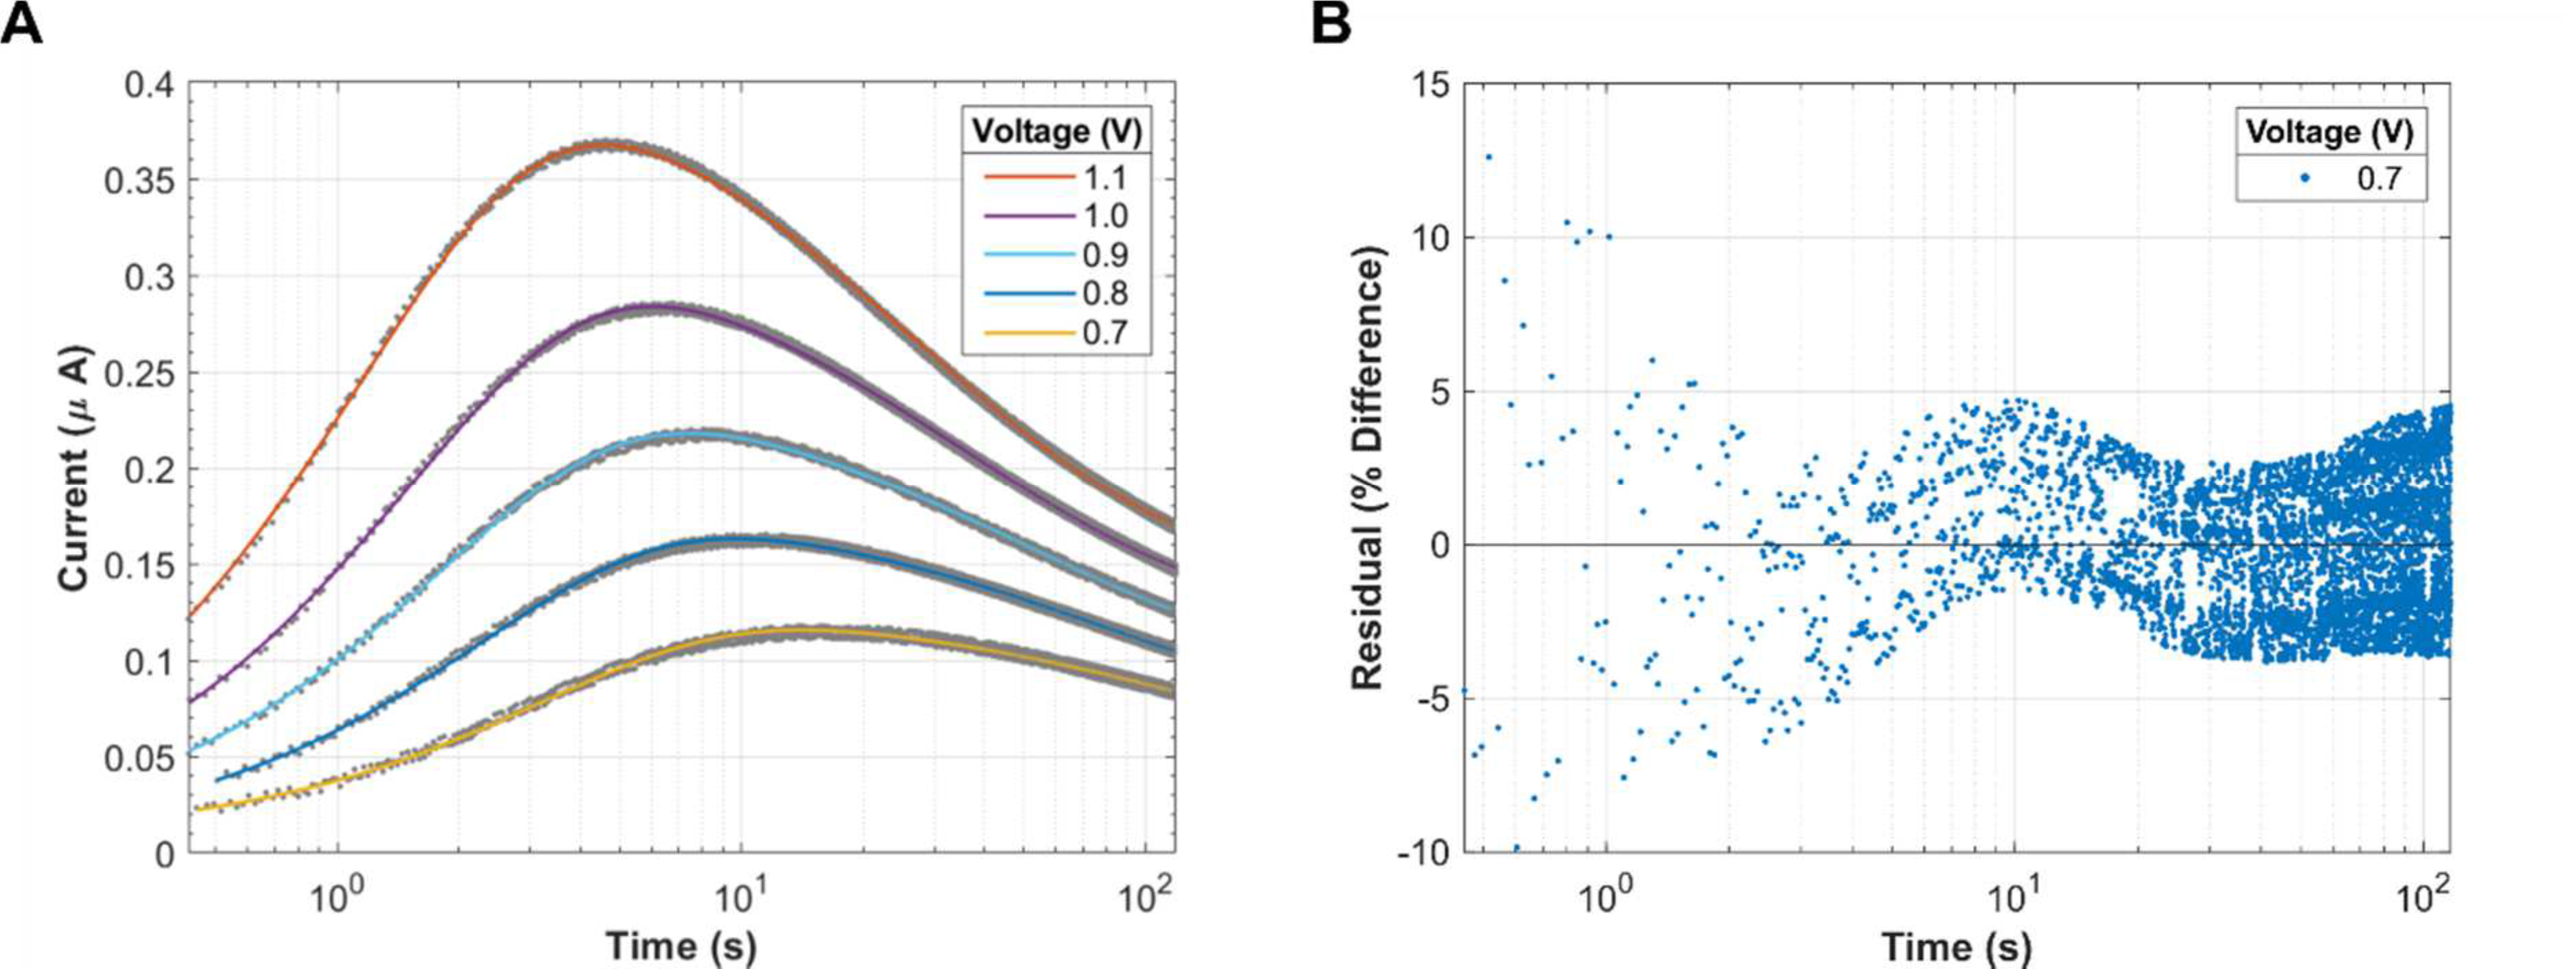
\includegraphics[width=1\textwidth]{Chapter6/Figs/e.png}
\caption[Single sweeps of 53 resistance states of a $SiO_x$ device.]{Single sweeps of 53 resistance states of a $SiO_x$ device. Different states were obtained by incrementing maximum voltage by 0.05V. Every seventh state shares the same colour; this does not indicate any other relationship between such states \cite{nikolaos_barmpatsalos_2021_5762184}.}
\label{fig:6e}
\end{figure}


\noindent The $SiO_x$ resistive random-access memory (RRAM) device comprised a $1 \mu m Si/SiO_2$  switching layer positioned between a 100nm $Mo$ bottom electrode and a 100nm $Au$ top electrode. Furthermore, a 5nm $Ti$ wetting layer was incorporated between the $SiO_x$ and $Au$ electrodes. Following electroforming and additional validation procedures, positive sweeps were conducted on the $SiO_x$ device, commencing from 0.5V and increasing by 0.05V in each run, thereby generating resistance states that spanned multiple orders of magnitude.\\

\noindent The majority of existing literature on ex-situ training of MNNs assumes a linear relationship between inputs and outputs at the level of individual devices. Non-linearities are only introduced at the level of the activation functions. In particular, outputs are assumed to be a function of the product of a vector of applied inputs and a matrix of weights:
\begin{align}
y_j = f\left( \sum_{i=1}^{M} x_i, w_{ij} \right) \label{eq:6.21}
\end{align}


\noindent Where the outputs, $y_j \in \textbf{y} \in \mathbb{R}^{1 \times N}$ is calculated using the inputs $x_i \in \textbf{x} \in \mathbb{R}^{1 \times M}$, weights $w_{ij} \in \textbf{w} \in \mathbb{R}^{M \times N}$, and a nonlinear activation function $f$. Non-Ohmic behaviour manifests itself in individual devices only, therefore these nonlinear effects can be separated from the other devices. To take I-V nonlinearities into account in ex-situ MNN training, the products in (\ref{eq:6.21}) can be replaced with a nonlinear function to give:
\begin{align}
y_j = f\left( \sum_{i=1}^{M} g \left( x_i, w_{ij} \right) \right) \label{eq:6.22}
\end{align}

\noindent In order to account for the non-ohmic behaviour of memristors, Function \textit{g} must be modified to reflect the specific characteristics of the mapping scheme between weights and conductances, as well as the non-ohmic device behaviour model, which is typically dependent on the type of devices employed \cite{joksas2022nonideality}.\\

\noindent The mapping scheme that relates weights and conductances is a crucial aspect to consider when designing memristive neural networks. In typical artificial neural networks, synaptic weights can assume any real value. Conversely, conductances are constrained to be non-negative.\\

\noindent To address this discrepancy, a neural network architecture was devised whereby twice the number of weights are trained, but each is constrained to be non-negative. This enables the association of weights with the conductances of individual devices, thereby creating a more natural mapping and facilitating adaptation to non-idealities. Additionally, it allows for more precise control over power consumption.\\

\noindent The aforementioned mappings are performed in an identical manner in the specific instance of fully connected synaptic layers in artificial neural networks, provided that conventional weight implementation methodologies are utilised. Both the inputs, designated as $x \in \mathbf{x}$, and the outputs, represented by $y \in \mathbf{y}$, are mapped onto voltages \textit{V} and total output currents \textit{I}, using the scaling factors $k_V$ and $k_I$, where $k_G$ is the conductance scaling factor:
\begin{align}
V &= k_V x \label{eq:6.23} \\
y &= \frac{I}{k_I} = \frac{I}{k_V k_G} \label{eq:6.24} \\
k_G &= \frac{G_{max} - G_{min}}{max |\mathbf{W}|} = \frac{G_{on} - G_{off}}{max |\mathbf{W}|}\label{eq:6.25}
\end{align}


\noindent  Irrespective of the scheme employed, a minimum of two conductances are required to encode both positive and negative weights. Conductances $G_+$ and $G_-$ are introduced into the "positive" and "negative" bit lines of the differential pair architecture, respectively. The proportionality of each weight is determined by the difference $G_+ - G_-$, with $k_G$ serving as the constant of proportionality. This enables the encoding of any real number within a finite range. In a typical differential pair implementation, $G_{min} = G_{off}$ and $G_{max} = G_{on}$. In an alternate proportional mapping scheme, $G_{min} = 0$ and $G_{max} = G_{on}$ to give $k_G = \frac{g_{on}}{max |\mathbf{W}|}$.\\

\noindent The issues associated with proportional mapping schemes, such as the presence of unimplementable regions, are not the only obstacles to be overcome. Conventional differential pair realisation also presents design challenges. For example, infinite conductance combinations will produce the same difference \cite{kim20214k}, i.e. the same effective conductance. \\

\noindent This means that an arbitrary choice may have to be made of how to perform the mapping between weights and conductances. To illustrate this, consider the encoding of weights $W \in \mathbf{W}$. In this case, pairs of conductances $G_+$ and $G_-$ may be picked symmetrically around the average value:
\begin{align}
G\pm &= G_{avg} \pm \frac{k_G w}{2} \label{eq:6.26} \\
G_{avg} &= \frac{G_{off} + G_{on}}{2} \label{eq:6.27}
\end{align}


\noindent While multiple mapping schemes may yield the same conductance difference, some may prove more advantageous than others. The scheme in (\ref{eq:6.26}) can be beneficial in certain scenarios, as it typically reduces the number of conductances near $G_{off}$ and $G_{on}$, which are often more challenging to achieve. However, the selection of the mapping scheme can be explicitly linked to specific objectives.\\

\noindent The differential pair architecture can be employed to mitigate the effects of stuck devices. To illustrate, if $G_+$ is stuck in an undesirable state, $G_-$ can be adjusted to minimise the negative effects. An alternative approach is to employ a simpler scheme that optimises a specific metric, such as power consumption. \\

\noindent This is illustrated in the simulations presented in this chapter, where conventional weights are used. In these simulations, a scheme that minimises power consumption is employed by ensuring that at least one of ${G_+, G_-}$ is set to $G_{off}$:
\begin{align}
G_+ &= G_{off} + max\left\{ 0, k_GW \right\} \label{eq:6.28} \\
G_- &= G_{off} - min\left\{ 0, k_GW \right\} \label{eq:6.29}
\end{align}

\noindent An alternative approach is to utilise two sets of non-negative weights, $W^+_{ij} \in \mathbf{W}_+ \in \mathbb{R}^{M \times N}_{\ge 0}$ and $W^-_{ij} \in \mathbf{W}_+ \in \mathbb{R}^{M \times N}_{\ge 0}$, which are collectively referred to as double weights \cite{kendall2020training}. This method entails mapping each weight onto a single conductance in the aforementioned "positive" and "negative" bit lines, respectively. \\

\noindent Despite the nonnegativity of each weight, the differential pair architecture allows for encoding the negative contribution of the $i_{th}$ input on the $j_{th}$ output through the introduction of a subtraction operation in hardware. Only the nonlinearity-aware node function in (\ref{eq:6.22}) requires adjustment to give:
\begin{align}
y_j = f\left( \sum_{i=1}^{M} g\left( x_i,W_{i,j}^+ \right) - g\left( x_i,W_{i,j}^- \right) \right) \label{eq:6.30}
\end{align}

\noindent As all weights in $\mathbf{W} := [W_+, W_-]$ are non-negative, they can be related to the corresponding conductances in the same way: $W_{\pm} \in [0, max(\mathbf{W})]$ can be linearly mapped onto $G_{\pm} \in [G_{off}, G_{on}]$, thus avoiding the introduction of weight gaps:
\begin{align}
G_{\pm} = k_GW_{\pm} + G_{off} \label{eq:6.31}
\end{align}

\noindent The initial benefit of utilising double weights is that the conductances are more directly exposed to the training algorithm. This enables the selection of combinations that achieve both optimal performance, for example in terms of loss and robustness. To illustrate, if specific non-idealities manifest more at lower conductance values, such as with programming deviations \cite{kim2016voltage}, the training may be able to select pairs at higher values, while maintaining the same difference between $G_+$ and $G_-$. This allows the minimisation of the negative effects of non-idealities without the need to explicitly specify which conductance pairs should be selected. \\

\noindent When weights \textit{W} are related to conductances \textit{G} in a monotonically increasing fashion (in this case, linear), regularisation can be employed to influence the magnitude of both weights and conductances. This provides a means of utilising regularisation as a high-level tool for controlling power consumption. It has been proposed that the \textit{L1} sparsification regulariser \cite{han2015learning} should be employed, as this has the potential to not only enhance training, for instance, by preventing overfitting, but also to promote lower conductance values. \\

\noindent In lieu of manually adjusting the mapping scheme, the network designer may elect to prioritize low power consumption to a greater or lesser extent. This may be determined by, for example, adjusting the regularisation factor in \textit{L1} regularisation and incorporated into the conventional hyperparameter tuning process  \cite{feurer2019hyperparameter}, which is typically performed before deploying SNNs in the real world.

\subsection[Nonidealities Calibrations]{Nonidealities Calibrations}

In the simulation presented in this chapter, a combination of experimental data from a $SiO_x$ device, models based on simplified assumptions regarding breaking-down devices, and findings from the literature on programming variability were employed. I-V nonlinearities have been identified as a prevalent method for characterising deviations from ohmic behaviour in memristive devices.
\begin{align}
\gamma \equiv \frac{G\left( 2V_{ref} \right)}{G\left( V_{ref} \right)}  \label{eq:6.32}
\end{align}

\noindent This approach involves the examination of two points on an I-V curve \cite{lentz2013current}, as previously discussed (\ref{eq:6.32}). This equation defines conductance linearity, which serves as a means of quantifying nonlinear I-V behaviour. A conductance linearity value of 1 is indicative of ohmic behaviour, while any deviation from this value indicates I-V nonlinearity. While this metric can be useful for describing non-ohmic behaviour at different voltages, it is more challenging to utilise for modelling purposes \cite{sung2018effect}.
\begin{align}
I & = V_{ref}G\left ( \frac{V}{V_{ref}} \right )^{log_2 \gamma} \label{eq:6.33}
\end{align}

\noindent In order to construct an I-V curve from a given nonlinearity parameter $\gamma$, it is possible to assume that the equality in Equation (\ref{eq:6.32}) holds for all $V$, rather than just $V_{ref}$. This would result in a relationship between current and voltage, as shown in (\ref{eq:6.32}). In this equation, $G$ represents the conductance parameter, which has a specific meaning in the context of $V_{ref}$, where the device produces the expected ohmic amount of current, which is equal to $V_{ref} G$.\\

\begin{figure}[htbp!] 
\centering    
\includegraphics[width=1\textwidth]{Chapter6/Figs/f.png}
\caption[I-V sweeps of a SiOx device are presented for two regions]{I-V sweeps of a SiOx device are presented for two regions: a) low-resistance region with average resistance ranging from 284.6 $\Omega$ to 1003 $\Omega$, and b) high-resistance region with average resistance ranging from 366.2 k$\Omega$ to 1.295 M$\Omega$. Only the voltage range from 0.0 V to 0.5 V was considered for all curves. The nonlinearity parameter was calculated by dividing the current at 0.5 V by the current at 0.25 V \cite{joksas2022nonideality}.}
\label{fig:6f}
\end{figure}


\noindent The nonlinearity parameters $\gamma$ were extracted from experimental data obtained from a $SiO_x$ RRAM device. $SiO_x$ devices are capable of undergoing resistance switching, which is characterised by a typical I-V switching curve. In order to achieve a wide range of resistance states and to analyse I-V nonlinearity, incremental positive sweeps were employed to gradually reset the device from the low-resistance state (LRS) to the high-resistance state (HRS). The low-resistance discrete states display greater linearity and exhibit minimal variability. Conversely, the high-resistance states are more nonlinear, and the nonlinearity is less predictable.\\

\noindent The value of $V_{ref}$ from (\ref{eq:6.32}), was set to 0.25V, which is equivalent to half of the minimum switching voltage. In each case, the devices could be set to any conductance between $G_{off} = 1/R_{off}$ and $G_{on} = 1/R_{on}$. The states for the two groups were selected in such a way that the $G_{on}/G_{off}$ ratio for high-resistance devices would be slightly larger. This approach ensures that any potential higher error rate in this group can be attributed to nonlinearity and its variability, rather than being attributed to limited dynamic range.\\

\noindent In order to guarantee more robust modelling, it was deemed necessary to take uncertainty regarding the degree of nonlinearity experienced by each device into account. Although there is a general tendency for high-resistance states to exhibit greater nonlinearity, the precise degree of nonlinearity at any given resistance state may be challenging to ascertain, as evidenced by the variability observed in the I-V curves depicted in the experimental data presented in Figure \ref{fig:6f}. \\

\noindent Consequently, for each device in either of the groups, the parameter $\gamma$ was drawn from a truncated normal distribution. This distribution was truncated for $\gamma$ values of less than 2, with the objective of ensuring realistic device behaviour and numerical stability of the simulations. The mean $m_\gamma$ and standard deviation $s_\gamma$, both of which refer to the underlying normal distribution prior to truncation, were used to characterise the distribution.\\

\noindent It is not possible to simulate nonidealities such as I-V nonlinearity using conventional noise injection methods that merely disturb the conductance values. Consequently, a forward propagation function must be defined in order to reflect the nonlinear relationship between inputs and outputs.
\begin{align}
g(x, w_\pm) = \frac{\left( k_Gw_\pm + G_{off}\right) \times \left( 2x \right)^{log_2\gamma_\pm}}{2k_G} \label{eq:6.34}
\end{align}

\noindent In the proposed training function, as outlined in Equation (\ref{eq:6.30}), the aforementioned I-V nonlinearity is incorporated into the function g by combining Equations (\ref{eq:6.25}), (\ref{eq:6.31}), (\ref{eq:6.33}), using $k_V = 2V_{ref}$ in accordance with the definition in Equation (\ref{eq:6.32}), resulting in the form presented in Equation (\ref{eq:6.34}). This function is then implemented using Keras.\\

\noindent In order to conduct simulations involving training, it is essential to utilise an I-V model that incorporates stochasticity. As a specific instance of nonlinear behaviour may be acquired during training, it is unclear how beneficial such a model would be when applied to a different set of devices. \\

\noindent It can be seen, therefore, that the previous approach may not be sufficient, since the experimental I-V measurements were used as a lookup table for computing currents of devices in certain conductance states at certain voltages. There are, however, multiple physical models that could be employed for describing non-ohmic memristor behaviour. \\

\noindent It was decided that the Poole-Frenkel conduction model \cite{joksas2022nonideality} would be the most appropriate to use, given that the underlying physical mechanism was deemed to be plausible for $SiO_x$ devices. Furthermore, the model demonstrated excellent fit to the experimental I-V curves. Its simple analytical form also allowed for the incorporation of stochasticity by considering the uncertainty in certain parameters.
\begin{align}
I = cV exp\left( \frac{2e}{k_BT} \sqrt{\frac{eV}{4\pi d\epsilon}} \right) \label{eq:6.35}
\end{align}

\noindent The Poole-Frenkel model postulates that the current through a device can be described by (\ref{eq:6.35}), where $I$ is the current, $V$ is the voltage, $c$ is a constant (with units of conductance), $T$ is the temperature which is 20 degrees Celsius, $d$ is the effective oxide thickness, and $\epsilon$ is the permittivity. Consequently, the parameter $c$ and the product $d\epsilon$ can be fitted.\\

\noindent In order to model the variability of $c$ and $d\epsilon$, an attempt was made to predict their values on the basis of observable variables. Deviations from any constructed trend would be indicative of the uncertainty in the values of these quantities. It has been demonstrated that memristive devices can behave differently in different resistance states \cite{mehonic2015structural}, and this phenomenon has often been linked to the conductance quantum $G_0 = 2e^2/h$ \cite{yi2016quantized}.\\

\noindent The variables $c$ and $d\epsilon$ serve to reiterate some of the observations made regarding the I-V behaviour of the $SiO_x$ device, thereby assisting in the assessment of the appropriateness of the Poole-Frenkel model. It was demonstrated that $c$ behaves in a manner analogous to that of conductance, specifically as the reciprocal of resistance \cite{joksas2022memristive}. The primary distinction between the lower- and higher-resistance states is that the discrepancies from the trend are markedly more pronounced in the latter. \\

\noindent In (\ref{eq:6.35}), the product $d\epsilon$ is indicative of the degree of nonlinearity. Given that this product appears in the denominator of an exponentiated square root, a smaller value of $d\epsilon$ corresponds to a more nonlinear I-V curve. In LRS, this product is significantly larger. Although this parameter algebraically (\ref{eq:6.35}) can approximate linear behaviour (i.e. ohmic conduction), the values of $d\epsilon$ are only plausible for the less conductive states proximate to and below $G_0$. \\

\noindent For higher-resistance states, this is less discernible. The $d\epsilon$ values are considerably lower for all such states, yet the trend is not only plateaued but also more erratic. This unpredictability is indicative of the diverse range of colours observed in the curves presented in Figure \ref{fig:6f}. While the significant deviations from the trend line may limit the applicability of this approach in conventional modelling scenarios, the inherent uncertainty is precisely what is required to assess the potential of ex-situ training in addressing unknown behaviours. \\

\noindent The individual data points were integrated into a statistical model that would facilitate the generation of as many data points as required. In order to evaluate the efficacy of the proposed training method, two distinct resistance regions were considered. The low-resistance range was constructed by means of interpolation of the model parameters between the lowest resistance state and five times that resistance. The high-resistance range was constructed by interpolating the model parameters between the highest resistance state and one-fifth of that resistance, to ensure that the dynamic range remained consistent. \\

\noindent The statistical model was employed to ascertain the output current of a given device in the following manner: the initial values of $c$ and $d\epsilon$ were interpolated from the pertinent fits using the resistance parameter $R$. Thereafter, $c$ and $d\epsilon$ were subjected to disturbance via a multivariate normal distribution, which took into account both sets of parameters. The covariance matrix was determined using the residuals of the fits, and the current I was determined using (\ref{eq:6.35}).\\

\noindent As previously stated, the selection of the output function g in ex-situ training with linearity-nonpreserving nonidealities is contingent upon both the mapping scheme and the intrinsic nature of the nonlinearity. The combination of a linear mapping between inputs and outputs (\ref{eq:6.25}), a double weights mapping (\ref{eq:6.26}), and the relationship between current and voltage characterised by $c$ and $d\epsilon$ (\ref{eq:6.35}); allows $g$ to be expressed as follows:
\begin{align}
g\left( x, W_\pm \right) &= \frac{cx\cdot exp\left( \frac{2e}{kbT} \sqrt{\frac{ek_Vx}{4\pi d\epsilon}} \right)}{k_G} \label{eq:6.36} \\
\begin{bmatrix} c \\  d\epsilon \end{bmatrix} &= exp\left( -ln\left( k_GW_\pm + G_{off} \right)\textbf{m} + \textbf{b} + \textbf{E} \right) \label{eq:6.37}
\end{align}

\noindent Where \textbf{m} is the slopes, \textbf{b} is the intercepts, and the error is drawn from a normal distribution $\textbf{E} \sim \mathcal{N}_2\left( 0, \Sigma \right)$, with 0 mean and standard deviation being the residual covariance matrix.

\section{Inference and Classification}

\subsection[Simulation Configurations]{Simulation Configurations}

\section[Summary]{Summary}